\documentclass{beamer}
\mode<presentation>
    {
      \usetheme{Madrid}
      \usecolortheme{default}
      \usefonttheme{default}
      \setbeamertemplate{navigation symbols}{}
      \setbeamertemplate{caption}[numbered]
    }
    
\usepackage[english]{babel}
\usepackage[utf8x]{inputenc}
\usepackage{graphicx}
\usepackage{subcaption}
\usepackage{pgf,tikz}
\usepackage{mathrsfs}
\usetikzlibrary{arrows}
\usefonttheme[onlymath]{serif}

\usepackage{listings}
\lstset{[language=C++,basicstyle=\ttfamily,keywordstyle=\color{red},xleftmargin=-25pt, xrightmargin=5pt}

\title[T. e I. de un Motor Gráfico]{Teoría e Implementación de un Motor Gráfico}
\author{Joel Pérez Ferrer}
\institute{Institut de Bruguers}
\date{3/11/2017}

\begin{document}

\begin{frame}
  \titlepage
\end{frame}

\section{Introducción}
\begin{frame}{El Motor Gráfico}
  Un \textbf{motor gráfico} son una serie de rutinas de programación que permiten el diseño, la creación y la representación de entornos interactivos como un videojuego.
  
\begin{figure} [h]
  \centering
  \captionsetup[subfigure]{justification=centering}
  \begin{subfigure}{0.4\textwidth}
    \centering
    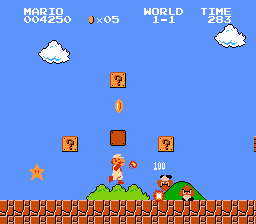
\includegraphics[width=0.8\textwidth]{img/supermario} 
    \caption{\textit{Super Mario Bros.} (1985)}
  \end{subfigure}
  \begin{subfigure}{0.4\textwidth}
    \centering
    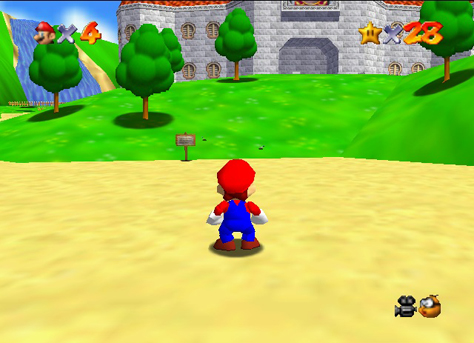
\includegraphics[width=0.8\textwidth]{img/mario64} 
    \caption{\textit{Super Mario 64} (1996)}
  \end{subfigure}
\end{figure}
\end{frame}


\begin{frame}{La Librería Gráfica}
  \begin{itemize}
  \item{La función de la librería gráfica ha ido cambiando a lo largo de los años.}
  \item{La \textbf{librería gráfica} que ha servido de inspiración ha sido OpenGL.}
  \end{itemize}
  \vfill
  \begin{figure}
    \centering
    
\includegraphics[width=0.5\textwidth]{img/OpenGL-Logo}
  \end{figure}
\end{frame}



\begin{frame}{Objetivos del Treball de Recerca}
  \begin{itemize}
    \item{Factibilidad de desarrollar una librería gráfica}
    \item{Factibilidad de desarrollar un motor gráfico}
    \item{Comprender el funcionamiento de un motor gráfico internamente}
    \item{Familiarizarse con herramientas de expresión científica}
  \end{itemize}
\end{frame}

\begin{frame}{Hipótesis}
  \begin{itemize}
    \item{Hipótesis original:}
  \end{itemize}
  \textit{Los equipos de desarrollo de software deberían de aspirar a ser ellos mismos quienes crean las herramientas que utilizarán para crear el software en sí, En caso de que esta sea una decisión no rentable, su máxima prioridad debería de ser entender cómo funcionan las herramientas que utilizarán.}
\end{frame}

\begin{frame}{Metodología}
  Un resultado final, muchas formas de llegar a él.
  \vfill
  \begin{figure} [h]
    \centering
    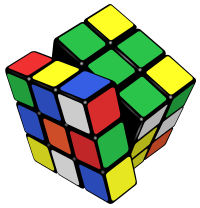
\includegraphics[width=0.3\textwidth]{img/rubik}
  \end{figure}
\end{frame}

\begin{frame}{Herramientas: Programación}
  \begin{itemize}
  \item{Lenguaje de Programación: C++ $\rightarrow$ \textbf{C/C++} $\rightarrow$ C++}
  \item{Compilador: \textbf{GNU Compiler Collection (GCC)}, MinGW GCC}
  \item{Editor de texto: \textbf{GNU Emacs}}
  \item{IDE: \textbf{Code::Blocks}}
  \item{Depurador: \textbf{GNU Project Debugger (GDB)}, interfaz GDB de Code::Blocks}
  \item{Sistema Operativo: \textbf{GNU/Linux}, MS Windows y macOS}
  \item{Gestor de código: \textbf{git} (\textit{Github})}
  \end{itemize}
  \begin{figure} [h]
    \centering
    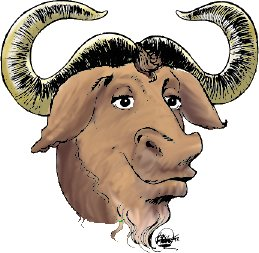
\includegraphics[width=0.2\textwidth]{img/reiss-head}
  \end{figure}
\end{frame}

\begin{frame}{Herramientas: Documentación}
  Tanto para el documento escrito como para en la presentación se han usado \textbf{las mismas herramientas}.
  \begin{itemize}
  \item{Lenguaje de Programación: \textrm{\LaTeX}}
  \item{Compilador: \textrm{\TeX  Live}}
  \item{Editor de texto: GNU Emacs}
  \item{Diagramas: Ti\textit{k}Z and PGF y GeoGebra}
  \end{itemize}
\end{frame}


\section{Teoria}
\begin{frame}{Espacio local}
  \begin{itemize}
  \item{Definición vértices}
  \item{Definición normales}
  \item{Antes de que ocurra cualquier transformación}
  \item{Coordenadas relativas al centro del objeto}
  \end{itemize}

  \begin{figure} [h!]
    \centering
    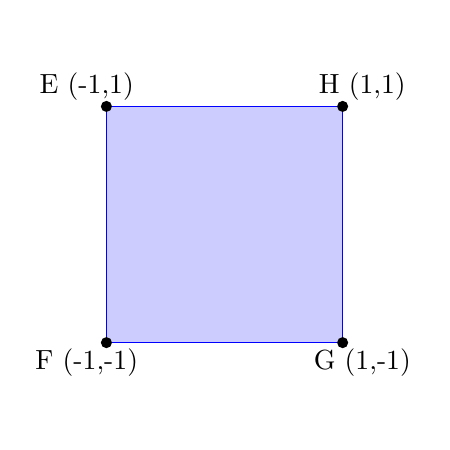
\begin{tikzpicture}
      \clip (0,0) rectangle (5,5);
      \draw [-,color=blue]
      (1,1) -- (4,1) -- (4,4) -- (1,4) -- (1,1);
      \fill [color=blue, opacity=0.2]
      (1,1) -- (4,1) -- (4,4) -- (1,4) -- (1,1);

      \draw
      (0.75,0.75) node {F (-1,-1)}
      (4.25,0.75) node {G (1,-1)}
      (4.25,4.25) node {H (1,1)}
      (0.75,4.25) node {E (-1,1)};

      \fill
      (1,1) circle (2pt)
      (4,1) circle (2pt)
      (4,4) circle (2pt)
      (1,4) circle (2pt);
      
    \end{tikzpicture}
  \end{figure}
  
\end{frame}

\begin{frame}{Implementación del espacio local I}
  \begin{figure} [ht]
  \centering
  \begin{tikzpicture}[thick, scale=0.4, every node/.style={scale=0.6}, line cap=round, line join=round, >=triangle 45, x=1cm, y=1cm]
    \clip(0,0) rectangle (6, 6);
    \draw(1,4) node (n0) {1};
    \draw(4,4) node (n1) {2};
    \draw(2,3) node (n2) {3};
    \draw(1,1) node (n3) {4};
    \draw(5,1) node (n4) {5};
    \draw(5,3) node (n5) {6};
    \end{tikzpicture}
  \caption*{GL\_POINTS}
\end{figure}


  \begin{figure} [h]
  \centering
  \captionsetup[subfigure]{justification=centering}
  \begin{subfigure}  {0.3\textwidth}
    \centering
    \begin{tikzpicture}[thick, scale=0.4, every node/.style={scale=1.2}, line cap=round, line join=round, >=triangle 45, x=1cm, y=1cm]
      \clip(0,0) rectangle (6, 6);
      (1,4) node (n0) {.};
      (4,4) node (n1) {.};
      (2,3) node (n2) {.};
      (1,1) node (n3) {.};
      (5,1) node (n4) {.};
      (5,3) node (n5) {.};

      \draw [-, line width=1pt, color=black]
      (n0.center) -- (n1.center)
      (n2.center) -- (n3.center)
      (n4.center) -- (n5.center);
      
    \end{tikzpicture}

    \caption{GL\_LINES}
  \end{subfigure}
  \begin{subfigure} {0.3\textwidth}
    \centering
    \begin{tikzpicture}[thick, scale=0.4, every node/.style={scale=1.2}, line cap=round, line join=round, >=triangle 45, x=1cm, y=1cm]
      \clip(0,0) rectangle (6, 6);
      (1,4) node (n0) {.};
      (4,4) node (n1) {.};
      (2,3) node (n2) {.};
      (1,1) node (n3) {.};
      (5,1) node (n4) {.};
      (5,3) node (n5) {.};

      \draw [-, line width=1pt, color=black]
      (n0.center) -- (n1.center)
      (n1.center) -- (n2.center)
      (n2.center) -- (n3.center)
      (n3.center) -- (n4.center)
      (n4.center) -- (n5.center);
      
    \end{tikzpicture}

    \caption{GL\_LINE\_STRIP}
  \end{subfigure}
  \begin{subfigure} {0.3\textwidth}
    \centering
    \begin{tikzpicture}[thick, scale=0.4, every node/.style={scale=1.2}, line cap=round, line join=round, >=triangle 45, x=1cm, y=1cm]
      \clip(0,0) rectangle (6, 6);
      (1,4) node (n0) {.};
      (4,4) node (n1) {.};
      (2,3) node (n2) {.};
      (1,1) node (n3) {.};
      (5,1) node (n4) {.};
      (5,3) node (n5) {.};

      \draw [-, line width=1pt, color=black]
      (n0.center) -- (n1.center)
      (n1.center) -- (n2.center)
      (n2.center) -- (n3.center)
      (n3.center) -- (n4.center)
      (n4.center) -- (n5.center)
      (n5.center) -- (n0.center);
      
    \end{tikzpicture}

    \caption{GL\_LINE\_LOOP}
  \end{subfigure}
\end{figure}

\end{frame}

\begin{frame}[fragile]{Implementación del espacio local II}
  Materialización del concepto del objeto como \textit{primitive}:
  \begin{lstlisting}[language=C++,basicstyle=\ttfamily,keywordstyle=\color{red},xleftmargin=-25pt,
      xrightmargin=5pt]
    glBegin(GLEnum mode);
  \end{lstlisting}
  \begin{lstlisting}[language=C++,basicstyle=\ttfamily,keywordstyle=\color{red},xleftmargin=-25pt,
      xrightmargin=5pt]
    glVertex3f(GLfloat x, GLfloat y, GLfloat z);
  \end{lstlisting}
  \begin{lstlisting}[language=C++,basicstyle=\ttfamily,keywordstyle=\color{red},xleftmargin=-25pt,
      xrightmargin=5pt]
    glColor3f(GLfloat r, GLfloat g, GLfloat b);
  \end{lstlisting}
  \begin{lstlisting}[language=C++,basicstyle=\ttfamily,keywordstyle=\color{red},xleftmargin=-25pt,
      xrightmargin=5pt]
    glEnd();
     
  \end{lstlisting}

\end{frame}

\begin{frame}[fragile]{Implementación del espacio local: un ejemplo}
  \begin{lstlisting}[frame=single, linewidth=0.52\textwidth, gobble=4, xleftmargin=90pt, xrightmargin=-90pt]
    glBegin(GL_LINE_STRIP);
    glVertex3f(-1, -1, 0);
    glVertex3f(-1,  1, 0);
    glVertex3f( 1,  1, 0);
    glVertex3f( 1, -1, 0);
    glEnd();
  \end{lstlisting}

    \begin{figure} [h!]
    \centering
    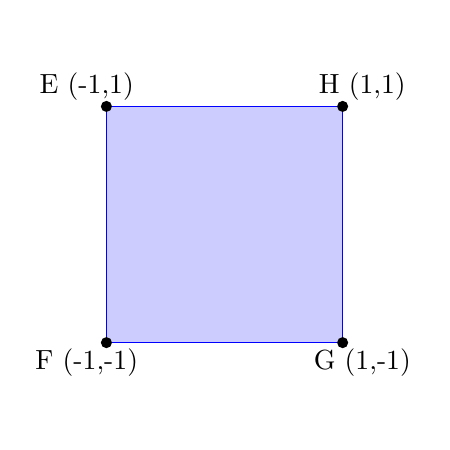
\begin{tikzpicture}
      \clip (0,0) rectangle (5,5);
      \draw [-,color=blue]
      (1,1) -- (4,1) -- (4,4) -- (1,4) -- (1,1);
      \fill [color=blue, opacity=0.2]
      (1,1) -- (4,1) -- (4,4) -- (1,4) -- (1,1);

      \draw
      (0.75,0.75) node {F (-1,-1)}
      (4.25,0.75) node {G (1,-1)}
      (4.25,4.25) node {H (1,1)}
      (0.75,4.25) node {E (-1,1)};

      \fill
      (1,1) circle (2pt)
      (4,1) circle (2pt)
      (4,4) circle (2pt)
      (1,4) circle (2pt);
      
    \end{tikzpicture}
  \end{figure}

\end{frame}

\begin{frame}{Implementación del espacio global y del espacio de vista}
  En OpenGL, la transformación de Modelo (espacio global) y la transformación de Vista (espacio de vista), ocurren a la vez.
  \begin{figure}[ht]
  \centering
  \(
  \begin{pmatrix}
    x_{vista}\\y_{vista}\\z_{vista}\\w_{vista}
  \end{pmatrix}
  = M_{modeloVista} \cdot
  \begin{pmatrix}
    x_{obj}\\y_{obj}\\z_{obj}\\w_{obj}
  \end{pmatrix}
  = M_{vista} \cdot M_{modelo} \cdot
  \begin{pmatrix}
    x_{obj}\\y_{obj}\\z_{obj}\\w_{obj}
  \end{pmatrix}
  \)
\end{figure}
\end{frame}

\begin{frame}{Espacio global}
  \begin{itemize}
  \item{Las coordenadas tienen valores absolutos respecto a un \textbf{punto arbitrario}.}
  \item{Pueden existir distintos objetos.}
  \end{itemize}

  \begin{figure}[h]
    \centering
    \definecolor{qqqqff}{rgb}{0,0,1}\definecolor{rvwvcq}{rgb}{0.08235294117647059,0.396078431372549,0.7529411764705882}\definecolor{cqcqcq}{rgb}{0.7529411764705882,0.7529411764705882,0.7529411764705882}\begin{tikzpicture}[line cap=round,line join=round,>=triangle 45,x=1cm,y=1cm]\draw [color=cqcqcq,, xstep=1cm,ystep=1cm] (-0.8954391833090678,4) grid (8.899624154736587,8.625717670298478);\draw[->,color=black] (0,3.5) -- (0,8.5);\foreach \y in {4,5,6,7,8}\draw[shift={(0,\y)},color=black] (2pt,0pt) -- (-2pt,0pt) node[left] {\footnotesize $\y$};\clip(-0.8954391833090678,1.7979314035066118) rectangle (7,9);\fill[line width=1pt,color=qqqqff,fill=qqqqff,fill opacity=0.15] (3,5) -- (6,5) -- (6,8) -- (3,8) -- cycle;\draw [line width=0.5pt,color=qqqqff] (3,5)-- (6,5);\draw [line width=0.5pt,color=qqqqff] (6,5)-- (6,8);\draw [line width=0.5pt,color=qqqqff] (6,8)-- (3,8);\draw [line width=0.5pt,color=qqqqff] (3,8)-- (3,5);\begin{scriptsize}\draw [fill=black] (3,5) circle (2pt);\draw[color=black] (3.0858504808186202,5.239292743321078) node {$M (3,5)$};\draw [fill=black] (6,5) circle (2pt);\draw[color=black] (6.085452282558659,5.239292743321078) node {$N (6,5)$};\draw [fill=black] (6,8) circle (2pt);\draw[color=black] (6.085452282558659,8.238894545061104) node {$O (6,8)$};\draw [fill=black] (3,8) circle (2pt);\draw[color=black] (3.0858504808186202,8.238894545061104) node {$P (3, 8)$};\end{scriptsize}\end{tikzpicture}
  \end{figure}

\end{frame}

\begin{frame}{Transformaciones}
  Una \textbf{transformación} puede ser toda función que mapea un conjunto $X$ en otro conjunto o sobre si mismo.
  \begin{itemize}
  \item{Translación}
  \item{Rotación}
  \item{Escalado}
  \end{itemize}
\end{frame}

\begin{frame}{Implementación de las transformaciones}
  \begin{figure}[ht]
  \centering
  \(
  \begin{pmatrix}
    \textcolor{red}{m_0} && \textcolor{green}{m_4} && \textcolor{blue}{m_8} && m_{12}\\
    \textcolor{red}{m_1} && \textcolor{green}{m_5} && \textcolor{blue}{m_9} && m_{13}\\
    \textcolor{red}{m_2} && \textcolor{green}{m_6} && \textcolor{blue}{m_{10}} && m_{14}\\
    \textcolor{gray}{m_3} && \textcolor{gray}{m_7} && \textcolor{gray}{m_{11}} && \textcolor{gray}{m_{15}}
  \end{pmatrix}
  \)
  \caption*{Matriz GL\_MODELVIEW}
\end{figure}
\begin{itemize}
\item{\((m_0, m_1, m_2)\) : eje +X, vector \textit{izquierda}, (1, 0, 0) por defecto}
\item{\((m_4, m_5, m_6)\) : eje +Y, vector \textit{arriba}, (0, 1, 0) por defecto}
\item{\((m_8, m_9, m_{10})\) : eje +Z, vector \textit{adelante}, (0, 0, 1) por defecto}
\end{itemize}
\end{frame}

\begin{frame}[fragile]{Translación}
  Una operación de translación consiste en desplazar un punto por un vector de coordenadas $(x, y, z)$.
  \begin{minipage}{0.3\textwidth}
  \centering
  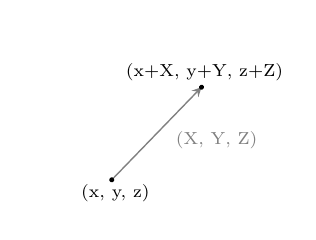
\begin{tikzpicture}[thick ,scale=0.6, every node/.style={scale=0.9}, line cap=round,line join=round,>=triangle 45,x=1cm,y=1cm]
    \clip(-7,-2.4) rectangle (-1.5,1.5);
    \draw [->,>=stealth,line width=0.5pt,color=gray] (-5.22,-1.72) -- (-3.32,0.24);
    \begin{scriptsize}
      \draw [fill=black] (-5.22,-1.72) circle (1pt);
      \draw[color=black] (-5.142466613438916,-2) node {(x, y, z)};
      \draw [fill=black] (-3.32,0.24) circle (1pt);
      \draw[color=black] (-3.2574601569280657,0.56) node {(x+X, y+Y, z+Z)};
      \draw[color=gray] (-3,-0.8810231214816775) node {(X, Y, Z)};
    \end{scriptsize}
  \end{tikzpicture}
  \end{minipage}\begin{minipage}{0.5\textwidth}
  \centering
  \[
  \begin{bmatrix}
    1 && 0 && 0 && X\\
    0 && 1 && 0 && Y\\
    0 && 0 && 1 && Z\\
    0 && 0 && 0 && 1
  \end{bmatrix}
  \cdot
  \begin{pmatrix}
    x \\ y \\ z \\ 1
  \end{pmatrix}
  =
  \begin{pmatrix}
    x + X \cdot 1 \\
    y + Y \cdot 1 \\
    z + Z \cdot 1 \\
    1
  \end{pmatrix}
  \]
  \end{minipage}
  \vfill
  \begin{lstlisting}
    glTranslatef(GLfloat x, GLfloat y, GLfloat z);
  \end{lstlisting}

\end{frame}

\begin{frame}{Rotación I}
  Una transformación de rotación rota un vector alrededor del origen $(0, 0, 0)$ utilizando un eje y un ángulo.

  \begin{figure} [ht!]
  \centering
  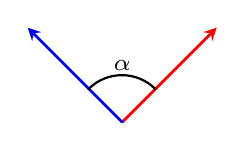
\begin{tikzpicture}[thick, scale=0.6, every node/.style={scale=1.2}, line cap=round, line join=round, >=triangle 45, x=1cm, y=1cm]
    \clip(-2, 0) rectangle (2, 2);
    \draw [->, >=stealth, line width=1pt, color=red] (0,0) -- (2, 2);
    \draw [->, >=stealth, line width=1pt, color=blue] (0,0) -- (-2, 2);
    \draw (0.702,0.702) arc[radius=1cm, start angle=45, end angle=(90+45)];
    
    \begin{scriptsize}
      \draw[color=black] (0, 1.2) node {$\alpha$};
    \end{scriptsize}
    
  \end{tikzpicture}
\end{figure}

  \begin{minipage}{0.4\textwidth}
  \centering
  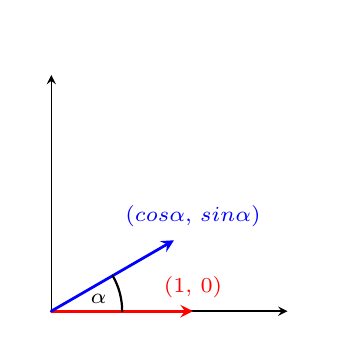
\begin{tikzpicture}[thick, scale=0.6, every node/.style={scale=1.1}, line cap=round, line join=round, >=triangle 45, x=1cm, y=1cm]
    \clip (-0.5, -0.5) rectangle (6, 6);
    \draw [->, >= stealth, line width=0.5pt, color=black] (0,0) -- (0, 5);
    \draw [->, >= stealth, line width=0.5pt, color=black] (0,0) -- (5, 0);
    \draw [->, >= stealth, line width=1pt, color=red] (0, 0) -- (3, 0);
    \draw [->, >= stealth, line width=1pt, color=blue] (0, 0) -- (2.598, 1.5);
    \draw (1.5 , 0) arc [radius =1.5cm, start angle=0, end angle=30];
    \begin{scriptsize}
      \draw[color=black] (1, 0.25) node {$\alpha$};
      \draw[color=red] (3, 0.5) node {(1, 0)};
      \draw[color=blue] (3, 2) node {($cos \alpha$, $sin \alpha$)};
    \end{scriptsize}
    \end{tikzpicture}
\end{minipage}
\begin{minipage}{0.5\textwidth}
  \centering
    \begin{tikzpicture}[thick, scale=0.6, every node/.style={scale=1.1}, line cap=round, line join=round, >=triangle 45, x=1cm, y=1cm]
    \clip (-6, -0.5) rectangle (6, 6);
    \draw [->, >= stealth, line width=0.5pt, color=black] (0,0) -- (0, 5);
    \draw [->, >= stealth, line width=0.5pt, color=black] (0,0) -- (5, 0);
    \draw [->, >= stealth, line width=0.5pt, color=black] (0,0) -- (-5, 0);
    \draw [->, >= stealth, line width=1pt, color=red] (0, 0) -- (0, 3);
    \draw [->, >= stealth, line width=1pt, color=blue] (0, 0) -- (-1.5, 2.598);
    \draw (0 , 1.5) arc [radius =1.5cm, start angle=90, end angle=120];
    \begin{scriptsize}
      \draw[color=black] (-0.25, 1) node {$\alpha$};
      \draw[color=red] (1, 2.5) node {(0, 1)};
      \draw[color=blue] (-2.7, 1.5) node {($-sin \alpha$, $cos \alpha$)};
    \end{scriptsize}
    \end{tikzpicture}
    
\end{minipage}

\end{frame}

\begin{frame}{Rotación II}
  Alrededor del eje Z:
  \begin{equation*}
  \begin{bmatrix}
    cos \alpha && -sin\alpha && 0 && 0 \\
    sin \alpha && cos\alpha && 0 && 0 \\
    0 && 0 && 1 && 0 \\
    0 && 0 && 0 && 1
  \end{bmatrix}
  \cdot
  \begin{pmatrix}
    x \\ y \\ z \\ 1
  \end{pmatrix}
  =
  \begin{pmatrix}
    cos \alpha \cdot x - sin \alpha \cdot y \\
    sin \alpha \cdot x + cos \alpha \cdot y \\
    z \\
    1
  \end{pmatrix}
  \end{equation*}
  Alrededor del eje X:
  \begin{equation*}
  \begin{bmatrix}
    1 && 0 && 0 && 0 \\
    0 && cos \alpha && -sin \alpha && 0 \\
    0 && sin \alpha && cos \alpha && 0 \\
    0 && 0 && 0 && 1
  \end{bmatrix}
  \cdot
  \begin{pmatrix}
    x \\ y \\ z \\ 1
  \end{pmatrix}
  =
  \begin{pmatrix}
    x \\
    cos \alpha \cdot y - sin \alpha \cdot z \\
    sin \alpha \cdot y + cos \alpha \cdot z \\
    1
  \end{pmatrix}
\end{equation*}
  Alrededor del eje Y:
  \begin{equation*}
  \begin{bmatrix}
    cos \alpha && 0 && sin \alpha && 0 \\
    0 && 1 && 0 && 0 \\
    - sin \alpha && 0 && cos \alpha && 0 \\
    0 && 0 && 0 && 1
  \end{bmatrix}
  \cdot
  \begin{pmatrix}
    x \\ y \\ z \\ 1
  \end{pmatrix}
  =
  \begin{pmatrix}
    cos \alpha \cdot x + sin \alpha \cdot z \\
    y \\
    - sin \alpha \cdot x + cos \alpha \cdot z \\
    1
  \end{pmatrix}
\end{equation*}

\end{frame}

\begin{frame}[fragile]{Rotación III}
  Tras la multiplicación de las anteriores matrices, se resulta en esta, que engloba las tres.
  \begin{figure} [ht]
  \centering
  \(
  \begin{pmatrix}
    x^2(1-c) + c  && xy(1-c) - zs && xz(1-c) + ys && 0\\
    xy(1-c) + zs && y^2(1-c) + c  && yz(1-c) - xs && 0\\
    xz(1-c) - ys && yz(1-c) + xs && z^2(1-c) + c  && 0\\
    0 && 0 && 0 && 1
  \end{pmatrix}
  \)
  \\donde $c = cos \alpha$, $s = sin \alpha$ 
  \caption*{Matriz de rotación, $M_R$}
  \end{figure}

  \begin{lstlisting}
    glRotatef(GLfloat angle,
              GLfloat x, GLfloat y, GLfloat z);
  \end{lstlisting}
\end{frame}

\begin{frame}[fragile]{Escalado}
  Una transformación de escalado consiste en escalar cada componente de un vector por un número.
  
  \begin{minipage}{0.3\textwidth}
  \begin{tikzpicture}[thick ,scale=0.6, every node/.style={scale=0.9}, line cap=round,line join=round,>=triangle 45,x=1cm,y=1cm]
    \clip(-3, -3) rectangle (3, 3);
    \draw [->,>=stealth, line width=0.5pt, color=blue] (-2,-2) -- (2,2);
    \draw [->,>=stealth, line width=0.5pt, color=red] (-2,-2) -- (0,0);
    \begin{scriptsize}
      \draw[color=red] (0,-1) node {(x, y, z)};
      \draw[color=blue] (2,0.8) node {(2x, 2y, z)};
      \draw[color=black] (1,-2) node {Escalar por (2,2,1)};
    \end{scriptsize}
  \end{tikzpicture}
\end{minipage}
\begin{minipage}{0.69\textwidth}
  \[
  \begin{bmatrix}
    SX && 0 && 0 && 0\\
    0 && SY && 0 && 0\\
    0 && 0 && SZ && 0\\
    0 && 0 && 0 && 1
  \end{bmatrix}
  \cdot
  \begin{pmatrix}
    x \\ y \\ z \\ 1
  \end{pmatrix}
  =
  \begin{pmatrix}
    SX \cdot x \\
    SY \cdot y \\
    SZ \cdot z \\
    1
  \end{pmatrix}
  \]
\end{minipage}
\begin{lstlisting} [xleftmargin=10pt]
  glScalef(GLfloat x, GLfloat y, GLfloat z);
\end{lstlisting}
\end{frame}

\begin{frame}{Espacio de clip}
  En este paso los objetos son transformados del espacio de vista al espacio de clip utilizando la matriz GL\_PROJECTION. Esta matriz se utiliza para definir el frustum o tronco de corte.
  \begin{figure}[ht]
    \centering
    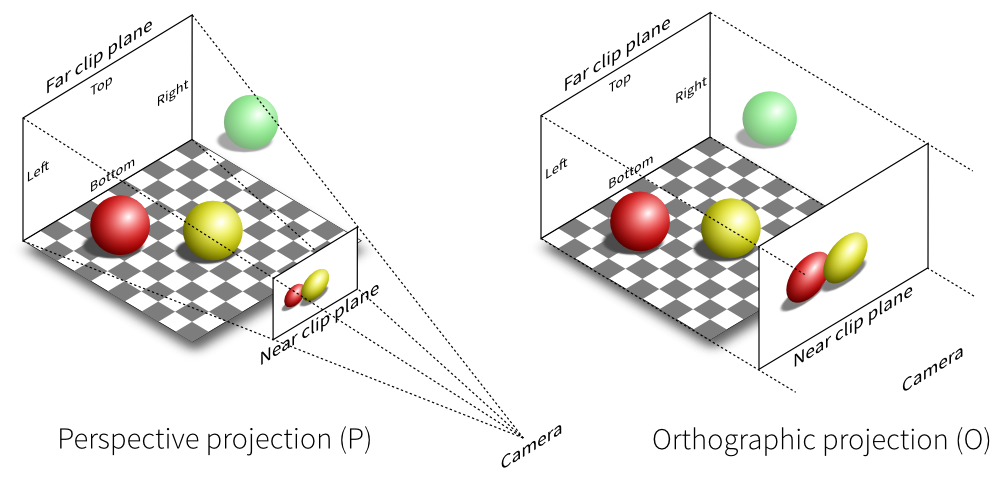
\includegraphics[width=0.7\textwidth]{img/projection}
  \end{figure}
\end{frame}

\begin{frame}{Espacio NDC}
  El espacio NDC (\textit{Normalized Device Coordinate}) es un espacio en el que las coordenadas que no han sido \textit{clipeadas} son escaladas dentro de un cubo de dimensiones $(-1, -1, -1)$ a $(1, 1, 1)$.

  \begin{figure}[h]
    \centering
    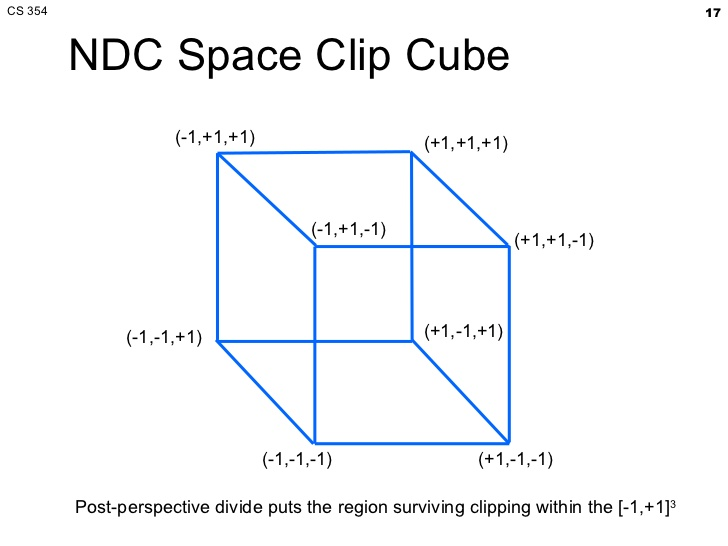
\includegraphics[width=0.6\textwidth]{img/ndc}
  \end{figure}
\end{frame}


\begin{frame}{Implementación del espacio de clip y del espacio NDC}
  \begin{itemize}
  \item{Primero, la información de las coordenadas de vista es transformada a coordenadas de clip.}
  \item{Después, estas coordenadas de clip son transformadas a NDC dividiendo por el componente $w$ de las coordenadas de clip.}
  \end{itemize}

  Por ello, tanto el clipping como las transformaciones NDC están integradas en la matriz GL\_PROJECTION.

  \begin{figure}[h]
    \centering
    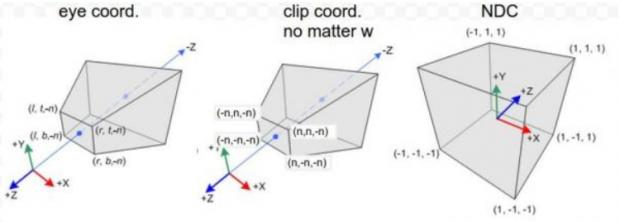
\includegraphics[width=0.6\textwidth]{img/clipspace}
  \end{figure}
  
\end{frame}

\begin{frame}{Proyección de perspectiva I}
  En una proyección de perspectiva, un punto 3D en un frustum piramidal truncado (coordenadas de vista) es mapeado a un cubo (NDC).
    \begin{figure}[h]
    \centering
    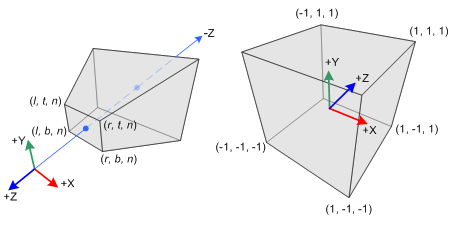
\includegraphics[width=0.5\textwidth]{img/gl_projectionmatrix01}
  \end{figure}

\end{frame}
\begin{frame}[fragile]{Proyección de perspectiva II}
  Una vez encontradas todas las entradas de la matriz GL\_PROJECTION, éste es el resultado.
  \begin{figure} [h]
  \(
  \begin{pmatrix}
    \frac{2n}{r-l} &&              0 &&   \frac{r+l}{r-l} &&                0 \\
                 0 && \frac{2n}{t-b} &&   \frac{t+b}{t-b} &&                0 \\
                 0 &&              0 && \frac{-(f+n)}{f-n} && \frac{-2fn}{f-n} \\
                 0 &&              0 &&                -1 &&                0
  \end{pmatrix}
  \)
  \caption*{Matriz de proyección de perspectiva de OpenGL}
  \end{figure}
  \begin{lstlisting}[xleftmargin=10pt]
    glFrustum(GLdouble left, GLdouble right,
              GLdouble bottom, GLdouble top,
              GLdouble near, GLdouble far);
  \end{lstlisting}
\end{frame}

\begin{frame}{Proyección ortográfica I}
  Construir la matriz GL\_PROJECTION para la proyección ortográfica es mucho más sencillo que para la proyección de perspectiva.
  \begin{figure}[h]
    \centering
    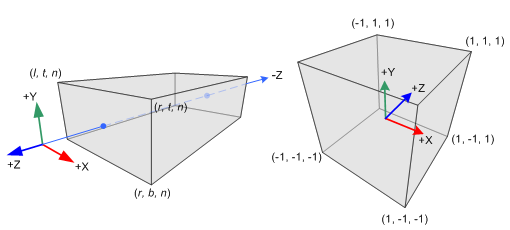
\includegraphics[width=0.5\textwidth]{img/gl_projectionmatrix02}
  \end{figure}
  Los componentes de los puntos en el espacio de vista son mapeados linearmente a NDC. Sólo es necesario escalar el volumen rectangular al cubo, y luego moverlo al origen.
\end{frame}
\begin{frame}[fragile]{Proyección ortográfica II}
  La matriz GL\_PROJECTION completa para la proyección ortográfica es la siguiente.
  \begin{figure} [h!]
  \(
  \begin{pmatrix}
    \frac{2}{r-l} &&             0 && - \frac{r+l}{r-l} &&                0 \\
                0 && \frac{2}{t-b} && - \frac{t+b}{t-b} &&                0 \\
                0 &&             0 &&    \frac{-2}{f-n} && -\frac{f+n}{f-n} \\
                0 &&             0 &&                  0 &&                1
  \end{pmatrix}
  \)
  \caption*{Matriz de proyección ortográfica de OpenGL}
\end{figure}
  \begin{lstlisting}[xleftmargin=10pt]
    glOrtho(GLdouble left, GLdouble right,
            GLdouble bottom, GLdouble top,
            GLdouble near, GLdouble far);
  \end{lstlisting}

\end{frame}


\begin{frame}{Espacio de ventana}
  En este paso, se pasará de las coordenadas normalizadas (NDC) al espacio de ventana, es decir, la imagen que se mostrará en pantalla finalmente.
  \begin{figure}[h]
    \centering
    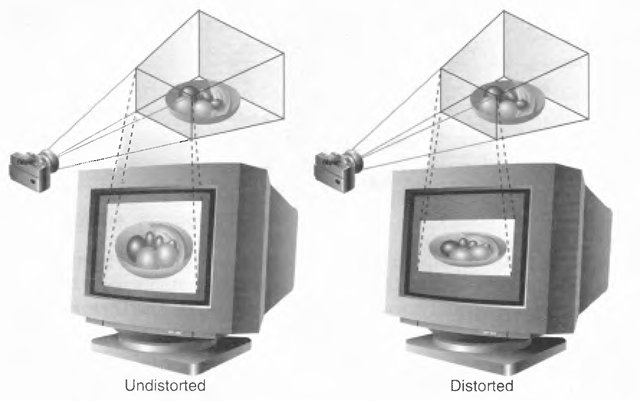
\includegraphics[width=0.5\textwidth]{img/viewport}
  \end{figure}
\end{frame}

\begin{frame}{Implementación del espacio de ventana I}
  Una vez se tienen las coordenadas normalizadas, encontrar la equivalencia en la pantalla es cuestión de escalar:
  \begin{equation*}
  \frac{x_s-(-1)}{1-(-1)} = \frac{x_d - x_m}{\Delta x}
  \end{equation*}
  Aislando $x_d$ se obtiene la siguiente expresión:
  \begin{equation*}
  x_d = \frac{\Delta x \cdot x_s}{2}+\frac{\Delta x}{2}+x_m
  \end{equation*}
  Para $y_d$ la expresión es similar, excepto que se cambia el sentido para conformar con el estándar.
  \begin{equation*}
  y_d = \frac{-(\Delta y) \cdot y_s}{2}+\frac{\Delta y}{2}+y_m
  \end{equation*}
\end{frame}

\begin{frame}{Implementación del espacio de ventana II}
  Y en forma de matriz, la operación resulta así:
  \begin{equation*}
  \begin{bmatrix}
     \frac{\Delta x}{2} && 0 && \frac{\Delta x}{2} + x_m\\
     0 && - \frac{\Delta y}{2} && \frac{\Delta y}{2} + y_m \\
     0 && 0 && 1
  \end{bmatrix}
  \cdot
  \begin{pmatrix}
    x_s\\
    y_s\\
    1
  \end{pmatrix}
  =
  \begin{pmatrix}
    x_d\\
    y_d\\
    1
  \end{pmatrix}
  \end{equation*}

  \vfill
  \begin{minipage}{0.5\textwidth}
    Mención importante a SDL:
  \begin{itemize}
  \item{Multiplataforma}
  \item{Sencillo}
  \item{Permite dibujar píxel a píxel}
  \end{itemize}

  \end{minipage}
  \begin{minipage}{0.4\textwidth}
    \begin{figure}[h]
    \centering
    
\includegraphics[width=0.6\textwidth]{img/SDL_logo}
    \end{figure}

  \end{minipage}

\end{frame}

\section{Conclusión}
\begin{frame}{Ajustes del método}
  \begin{figure}[h]
    \centering
    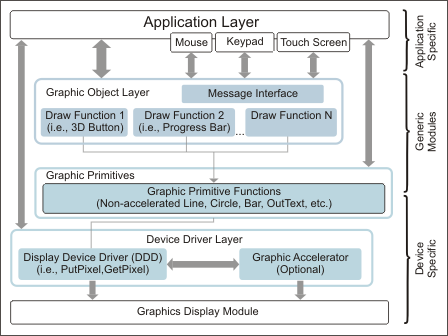
\includegraphics[width=0.7\textwidth]{img/method}
  \end{figure}

\end{frame}
\begin{frame}{Revisión de la hipótesis}
  Un mismo problema, dos soluciones opuestas.
  \vfill
  \begin{minipage}{0.45\textwidth}
    \centering
    \begin{figure}[h]
      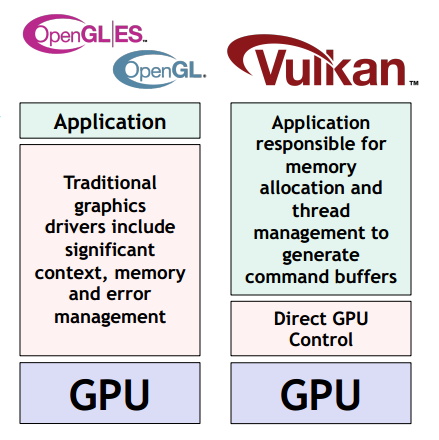
\includegraphics[width=0.8\textwidth]{img/vulkan_info}
    \end{figure}
  \end{minipage}
  \begin{minipage}{0.45\textwidth}
    \centering
    \begin{figure}[h]
      
\includegraphics[width=0.8\textwidth]{img/engines}
    \end{figure}
    \end{minipage}
\end{frame}
\begin{frame}{Preguntas}
\end{frame}
\begin{frame}{Valoración personal}
\end{frame}

\end{document}
